\documentclass[a4paper,12pt]{article}

%Class
	%\documentclass[a4paper,12pt]{article}

%Packages
	\usepackage{amsmath}					% Standard maths
	\usepackage{amssymb}					% Standard maths
	\usepackage{amsthm}						% Standard maths
	\usepackage{thmtools, thm-restate}% Theorem styles
	\usepackage{mathtools}
	\usepackage[newzealand]{babel}% Date/time in British format (yes, I know it says NZ)
	\usepackage{datetime}					% Date/time
	\usepackage{multirow}					% For stacked subscripts
	\usepackage{xcolor}						% For colour!
	\usepackage[normalem]{ulem}		% For strikeout
	\usepackage{isomath}
	\usepackage{fancyhdr}					% For the headers
	\usepackage{mfirstuc}					% For the headers
	\usepackage[hmargin=1in,top=0.8in,bottom=1in]{geometry} % Page margins more reasonable
	\usepackage{graphicx}					% For including graphics
	%\usepackage{float}						% For something
	\usepackage{enumitem}					% For numbering tweaks
	\usepackage{pgfplots}
	\usepackage[margin=15pt,font={footnotesize},labelfont=bf,format=hang]{caption}
\usepackage[margin=15pt,font={footnotesize},labelfont=bf,format=hang]{subcaption}
	\usepackage{url}
	\usepackage[hidelinks]{hyperref}	% For hyperlinks
	\usepackage{breakurl}
	\usepackage{cleveref}
	\usepackage[scaled=.92]{helvet}
	\newbool{show_question}
	\newbool{show_solution}
	\newcommand{\solutioninheading}{\ifbool{show_solution}{: SOLUTIONS}{}}
	\usepackage{pgfplots}
\newcommand{\ep}{\varepsilon}

\makeatletter 
\newcommand\mynobreakpar{\par\nobreak\@afterheading} 
\makeatother

    \newcommand{\question}[3]{
    	\item \textbf{#1} \mynobreakpar \nobreak \medskip % Title
    	%
    	\ifbool{show_question}{\nobreak#2}{} % Question
    	%
    	%
    	\ifbool{show_question}{\ifbool{show_solution}{\par\medskip\textbf{Solution:}}{}}{} % Both
    	\ifbool{show_solution}{#3}{} % Answer
    }			

%MATHEMATICAL SHORTCUTS
%Two and three-part definitions
	\newcommand{\twopartdef}[4]
	{	\left\{
			\begin{array}{ll}
				#1 & \mbox{if } #2 \\
				#3 & \mbox{if } #4
			\end{array}
		\right.}
%	\newcommand{\threepartdef}[6]
%	{	\left\{
%			\begin{array}{ll}
%				#1 & \mbox{if } #2 \\
%				#3 & \mbox{if } #4 \\
%				#5 & \mbox{if } #6
%			\end{array}
%		\right.}
%Blackboard bold	
	\newcommand{\N}{{\mathbb N}} 
	\newcommand{\R}{{\mathbb R}} 
	\newcommand{\C}{{\mathbb C}} 
	%Curly letters
%	\newcommand{\E}{{\mathcal E}}	
%	\newcommand{\F}{{\mathcal F}} 
%	\newcommand{\Null}{{\mathcal N}} 
%	\newcommand{\R}{\mathcal{R}} 
%	\newcommand{\Z}{\mathcal{Z}} 
%Uprights
	\newcommand{\D}{{\mathrm D}}
	\renewcommand{\d}{{\mathrm d}}
%Easy Greeks
%	\def\a{\alpha}
%	\def\g{\gamma}
%	\newcommand{\e}{{\varepsilon}}
%	\newcommand{\la}{{\lambda}}  
%	\newcommand{\om}{{\Omega}}
	\renewcommand{\epsilon}{\varepsilon}
	
%Vector operators
	\def \p {\partial}
	\newcommand{\del}{{\nabla}}
	\newcommand{\grad}{{\nabla}}
    \newcommand{\vdel}{\boldsymbol{\nabla}}
    \newcommand{\vgrad}{\boldsymbol{\nabla}}
    \newcommand{\vnabla}{\boldsymbol{\nabla}}
	\newcommand{\cross}{{\times}}
	\newcommand{\Lap}{{\nabla^2}} 
%Arrows
%	\newcommand{\goesto}[1]{\xrightarrow[#1]{}}
%hats
%	\newcommand{\nhat}{\widehat{\v{n}}}
%	\newcommand{\shat}{\widehat{\v{s}}}
	\renewcommand{\hat}{\widehat}
%Note to self
%	\newcommand{\note}[1]{[\textbf{\textsl{\MakeUppercase{#1}}}]}
	
%Stress tensor
%	\newcommand{\T}{\vg{\sigma}}

% Vectors, quaternions etc.
\renewcommand{\v}[1]{\mathbfit{#1}}      % Generic vector
\newcommand{\vc}[1]{\bm{\mathcal{#1}}}      % vector mathcal
\newcommand{\uv}[1]{\widehat{\mathbfit{#1}}}      % Generic unit vector
\newcommand{\q}[1]{\mathsfbfit{#1}}        % Generic quaternion
\renewcommand{\t}[1]{\mathsfbfit{#1}}	 % Generic tensor
\newcommand{\m}[1]{\mathsfbfit{#1}}	 % Generic matrix
\newcommand{\vu}[1]{\mathbf{#1}}         % Upright vector (for zero vector)
\newcommand{\qu}[1]{\mathbf{#1}}       % Upright quaternion (for zero quaternion)
\newcommand{\tu}[1]{\bm{\mathsf{#1}}}	 % Upright tensor (for zero tensor)

%Real and imaginary
\renewcommand{\Re}{\operatorname{Re}}
\renewcommand{\Im}{\operatorname{Im}}
	
%Non-dim numbers
%	\renewcommand{\Re}{\operatorname{Re}}
%	\newcommand{\Bi}{\operatorname{Bi}}
%	\newcommand{\Fo}{\operatorname{Fo}}
	
%Misc
\DeclareMathSymbol{\Delta}{\mathalpha}{operators}{1} % Keeps Delta upright
\DeclareMathSymbol{\Gamma}{\mathalpha}{operators}{0} % Keeps Gamma upright
	\newcommand{\cosec}{\operatorname{cosec}}
	\newcommand{\cosech}{\operatorname{cosech}}
	\newcommand{\sech}{\operatorname{sech}}
	\newcommand{\tr}{\operatorname{tr}}
	\newcommand{\erf}{\operatorname{erf}}
	\newcommand{\order}{\mathcal{O}}
%	\newcommand{\V}{\mathcal{V}} % 	CurlyV = (Bi V) / (1 + Bi)

% Differentiating 
\newcommand{\fd}[2]{\mathchoice{\frac{\d #1}{\d #2}}{\d #1/\d #2}{\d #1/\d #2}{\d #1/\d #2}}
\newcommand{\fdd}[2]{\mathchoice{\frac{\d^2 #1}{\d #2^2}}{\d^2 #1/\d #2^2}{\d^2 #1/\d #2^2}{\d^2 #1/\d #2^2}}
\newcommand{\fddd}[2]{\mathchoice{\frac{\d^3 #1}{\d #2^3}}{\d^3 #1/\d #2^3}{\d^3 #1/\d #2^3}{\d^3 #1/\d #2^3}}
\newcommand{\fdddd}[2]{\mathchoice{\frac{\d^4 #1}{\d #2^4}}{\d^4 #1/\d #2^4}{\d^4 #1/\d #2^4}{\d^4 #1/\d #2^4}}
\newcommand{\fdn}[3]{\mathchoice{\frac{\d^{#1} #2}{\d #3^{#1}}}{\d^{#1} #2/\d #3^{#1}}{\d^{#1} #2/\d #3^{#1}}{\d^{#1} #2/\d #3^{#1}}}
\newcommand{\pd}[2]{\mathchoice{\frac{\p #1}{\p #2}}{\p #1/\p #2}{\p #1/\p #2}{\p #1/\p #2}}
\newcommand{\pdd}[2]{\mathchoice{\frac{\p^2 #1}{\p #2^2}}{\p^2 #1/\p #2^2}{\p^2 #1/\p #2^2}{\p^2 #1/\p #2^2}}
\newcommand{\pddmixed}[3]{\frac{\p^2 #1}{\p #2 \p #3}}
\newcommand{\pddd}[2]{\frac{\p^3 #1}{\p #2^3}}
\newcommand{\pdn}[3]{\mathchoice{\frac{\p^{#1} #2}{\p #3^{#1}}}{\p^{#1} #2/\p #3^{#1}}{\p^{#1} #2/\p #3^{#1}}{\p^{#1} #2/\p #3^{#1}}}
	
	% Misc
\newcommand{\e}{\mathrm{e}}
\renewcommand{\i}{\mathrm{i}}
\newcommand{\dx}{\,\mathrm{d}x}
\newcommand{\dy}{\,\mathrm{d}y}
\renewcommand{\epsilon}{\varepsilon}
\renewcommand{\Re}{\operatorname{Re}}
\newcommand{\Four}{\mathcal{F}}

\newcommand{\mat}[4]{\begin{pmatrix}#1 & #2 \\ #3 & #4 \end{pmatrix}}

	%Column vectors
	\makeatletter
\newcommand\rcvector[2][\\]{\ensuremath{%
  \global\def\rc@delim{#1}%
    \negthinspace\begin{pmatrix}
      \rc@vector #2,\relax\noexpand\@eolst%
    \end{pmatrix}}}
\def\rc@vector #1,#2\@eolst{%
  \ifx\relax#2\relax
    #1
  \else
    #1\rc@delim
    \rc@vector #2\@eolst%
  \fi}
\makeatother

\newcommand{\colvec}{\rcvector}
\newcommand{\rowvec}{\rcvector}
\renewcommand{\binom}{\rcvector}
	
	%Colours
%	\newcommand{\orange}[1]{{\color{orange} #1 }}
%	\newcommand{\blue}[1]{{\color{blue} #1 }}

%Theorem styles
%	\declaretheoremstyle[headpunct={\:\:\:}, shaded={bgcolor={rgb}{0.9,0.9,0.9}, margin=5pt}]{problem}
%	\declaretheoremstyle[headpunct={\:\:\:}, shaded={rulecolor=black, rulewidth=0.4pt, bgcolor={rgb}{1,1,1}, margin=5pt}]{definition}
%	\declaretheoremstyle[headpunct={\:\:\:}, spaceabove=15pt, notefont=\bf, notebraces={(}{)}]{theorem}
%	\declaretheoremstyle[headpunct={\:\:\:}, numbered=no, spaceabove=15pt, qed={\checkmark}]{solution}
%	
%	\declaretheorem[style=definition,numberwithin=section]{definition}
%	\declaretheorem[numberlike=definition, style=theorem]{theorem}
%	\declaretheorem[numberlike=definition, style=theorem]{lemma}
%	\declaretheorem[numberlike=definition,style=problem]{problem}
%	\declaretheorem[numberlike=definition, style=theorem]{proposition}
%	\declaretheorem[numberlike=definition, style=theorem]{corollary}
%	\declaretheorem[numberlike=definition, style=theorem]{remark}
%	\declaretheorem[numberlike=definition, style=theorem]{example}
%	\declaretheorem[numberlike=definition, style=theorem]{notation}
%	\declaretheorem[style=solution]{solution}

%Depth of display breaks to allow	
	\allowdisplaybreaks[1]

%How deep do we want the Table of Contents to go?	
%	\setcounter{tocdepth}{1}

%Sections
\makeatletter
\renewcommand{\section}{\@startsection
{section}%                   % the name
{1}%                         % the level
{0mm}%                       % the indent
{-\baselineskip}%            % the before skip
{0.5\baselineskip}%          % the after skip
{\normalfont\bfseries}} % the style
\makeatother

% Wavy underline
\makeatletter
\font\sixly=lasyb10 scaled 1200
\def\tinners{\bgroup \markoverwith{\lower8.5\p@\hbox{\sixly \char58}}\ULon}
\makeatother
\newcommand{\answer}[1]{\tinners{\; #1 \;}}

%Setting the footnotes to use *,**,+ etc rather than 1,2,3	
\renewcommand{\thefootnote}{\fnsymbol{footnote}}

%Italic quote environment
%\newenvironment{quoteitalic}{\begin{quote}\itshape}{\end{quote}}

%Heading
\newcommand{\heading}[2]{
\setlength{\parindent}{0pt}
\textbf{MATH3171 (Mathematical Biology III)}

\textbf{YEAR 2025--26, \MakeUppercase{#1} TERM}
\setlength{\parskip}{3ex}

\textbf{\MakeUppercase{#2}}
%
\setlength{\parskip}{2ex}

}

%========================================================================================================================
%DOCUMENT BEGINS HERE!

\begin{document} 
%
\heading{Epiphany}{Problems class 8}
%\heading{Epiphany}{Problems class 8: solutions}
\newcommand{\sol}[1]{}
%\newcommand{\sol}[1]{\\ \hrule\hfill \\ \textcolor{blue}{\textbf{SOLUTION:}} #1 \\ \hrule\hfill}
\renewcommand*{\thefootnote}{\arabic{footnote}}

\section*{Turing analysis \& polar reaction--diffusion equations}
    
    \begin{enumerate}
\item{
\textbf{Turing analysis of predator--prey systems} \quad 
Consider the following reaction diffusion system modelling a predator $v$ and a prey $u$:
\begin{equation}
\label{sys1}
\begin{aligned}
\pd{u}{t}  &= \pdd{u}{x} + u(1-u)-g(u)v,\\
\pd{v}{t}  &= D\pdd{v}{x} + ag(u)v-bv,
\end{aligned}
\end{equation}
on the domain $x \in [0,L]$ with Neumann boundary conditions for both species. Here $D$ is the ratio of diffusion constants, $a$ and $b$ are positive constants, and $g$ is a function representing a \emph{density-dependent functional response} of the rate at which a predator consumes a prey. We assume that $g(0)=0$ and that $g$ is monotonically increasing. Hence, for any $c>0$, there is a unique\footnote{You could relax this technical assumption. It's worth thinking about how, e.g., the number of steady states changes if $g$ only takes values in an interval $[0,d]$ or $[0,d)$ for some positive number $d$, or if $g$ is non-monotonic (draw pictures!) Don't worry about this for this problems class. } $u_0$ satisfying $g(u_0)=c$.
\begin{enumerate}
\item{Determine the homogeneous equilibria of \eqref{sys1}. Besides $a>0$ and $b>0$, what additional assumptions, if any, are needed for these steady states to be feasible (that is, non-negative)?
\sol{There are two predator-free equilibria given by $(u_0,v_0)=(0,0),(1,0)$. Using the assumption on $g$, we know that there is a unique $u_0$ such that $g(u_0)=b/a$. We then have by the first equation that $v_0 = au_0(1-u_0)/b$. We have that $u_0>0$ by assumptions on $g$, but we require that $u_0 \in (0,1]$ for $v_0$ to be feasible. We can also spot that if $u_0=1$, $v_0=0$ which is a different equilibrium, so to have three distinct equilibria we need $u_0 \in (0,1)$.}
\item{In two of the equilibria above, one or both species densities is zero. Would it make biological sense to have a Turing instability around such a homogeneous equilibrium? Hint: Consider the eigenfunctions corresponding to an inhomogeneous perturbation, and think about if this would be physically sensible as an initial state of the population.
\sol{As suggested in the hint, we can write the eigenfunctions for the Laplacian as,
$$
w_k(x) = \cos\left(\frac{k\pi x}{L} \right).
$$
An inhomogeneous perturbation is one for which $k\geq 1$. Since these will be perturbations of an equilibrium which is zero, then in some part of the domain the perturbation would have a negative density. Hence these perturbations are in fact forbidden if we are considering an equilibrium with a zero component.

So the only equilibrium which it would make sense to do a Turing analysis around is the nonzero one given by $(u_0,v_0) = (u_0,au_0(1-u_0)/b)$ where $u_0$ satisfies $g(u_0)=b/a$.

NB (not examinable, just for your interest): This isn't just a biological impasse -- we can mathematically formalize this notion as the set of functions with $u \geq 0$ and $v \geq$ forms an `invariant region' of the dynamics, so we do not need to consider perturbations which violate this invariance. }
}
\item{Consider now only the equilibrium which can admit a Turing instability. Compute the Jacobian matrix (you do not need to substitute in values for $(u_0, v_0)$). Using the assumptions on the function $g$, and the properties of the equilibrium you have found,  determine whether this Jacobian can be of the right sign structure as required for a Turing instability.}
\sol{The Jacobian is given by,
$$
\m{J} = \begin{pmatrix} 1-2u_0-g'(u_0)v_0  & -g(u_0)\\ ag'(u_0)v_0 & ag(u_0)-b
\end{pmatrix}.
$$
As $g$ is monotonically increasing, we have $g'(u_0)>0$, so the top-right and bottom-left components have negative and positive signs, respectively. The top-left component is trickier, and will depend on the value of $g'(u_0)$. However, the bottom-right component is identically zero - note what equation $u_0$ has to satisfy to see this. The requirements of the sign structure of the Jacobian are strict positive or negative values at the equilibrium. So a zero means that if the homogeneous equilibrium is stable in the absence of diffusion, it must remain stable even with diffusion.

Hence, none of these equilibria can exhibit a Turing instability.
}
}
\end{enumerate}
}
%Q2
\item \textbf{Bacterial growth in a Petri dish}
Consider the growth of a colony of \emph{Escherichia coli} (often called \emph{E.\ coli}) in a circular container known as a \emph{Petri dish}. See Figure \ref{Petri}. We assume that there is plentiful food throughout the dish, but an antibiotic at the walls, which immediately kills any bacteria which touches the edge of the dish.

\begin{figure}
    \centering
    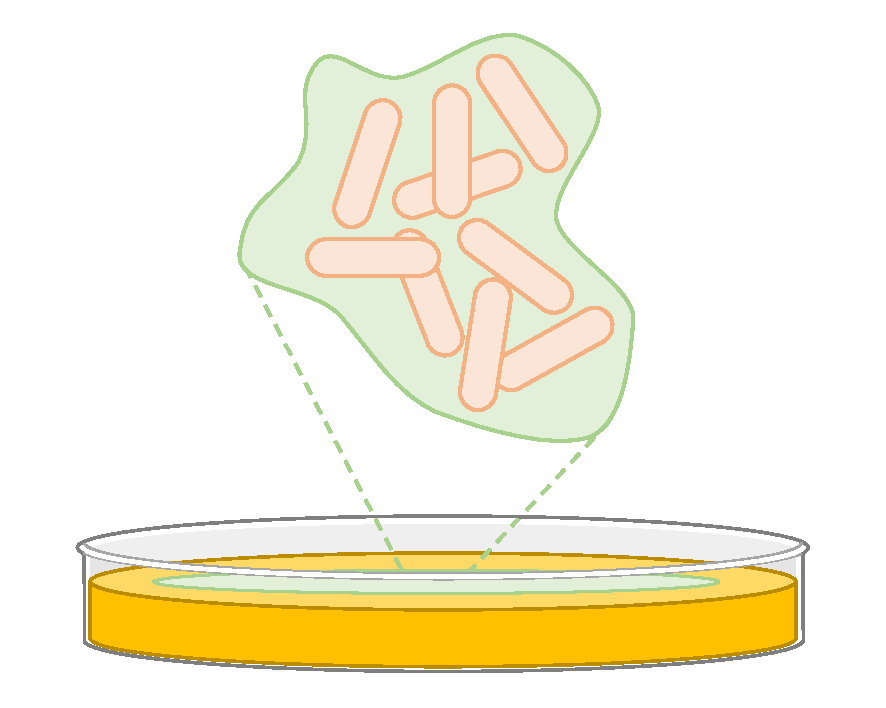
\includegraphics[width=0.45\textwidth]{Fig1aCells_Agar}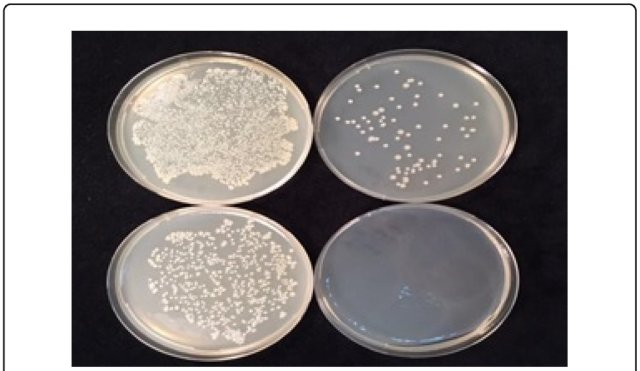
\includegraphics[clip, trim = 1cm 0 1cm 0.5cm, width=0.47\textwidth]{Petri}
    \caption{A diagram of \emph{E.\ coli} in a Petri dish. Typically they grow in a single large colony called a biofilm which is well-approximated as a two-dimensional structure. If food is scarce, these colonies can break apart as in the right panel.}
    \label{Petri}
\end{figure}

We model this using a two-dimensional reaction-diffusion equation,
\begin{equation}
    \pd{u}{t} = D\nabla^2 u + u(1-u),
\end{equation}
where $D$ is a scaled diffusion coefficient. We have non-dimensionalized the bacterial density $u$ and timescale $t$ such that the carrying capacity of the culture medium (the bacteria's food source) is $1$, and that the growth rate is also $1$. Our domain is the two-dimensional disc $(r,\theta)$ with $r\in [0, L_r]$ the radial coordinate, and $\theta\in [0, 2\pi)$ the angular coordinate. In this polar coordinate system the Laplacian takes the form
\begin{equation}
\nabla^2u  = \frac{1}{r}\pd{}{r}\left(r \pd{u}{r}\right) + \frac{1}{r^2}\pdd{u}{\theta}.
\end{equation}
We have the boundary conditions
\begin{equation}
    {u}(t,L_r,\theta) = 0,\qquad {u}(t,r,0) ={u}(t,r,2\pi),\qquad  \pd{u}{\theta}(t,r,0) = \pd{u}{\theta}(t,r,2\pi).
\end{equation}
The first of these represents bacterial death at the walls, and the second two are periodic conditions conditions in $\theta$.
\begin{enumerate}
    \item What are the permissible homogeneous equilibria of this model? Remember -- these must satisfy the boundary conditions!
    \sol{As we have $u(r=L_r)=0$, the only permissible homogeneous equilibrium is $u_0=0$.}
    \item Write the linear equation governing perturbations of a homogeneous equilibrium. 
    \sol{We have the linear equation as,
    $$
        \pd{u_1}{t} = D\nabla^2 u_1 + u_1(1-2u_0) = D\nabla^2 u_1 + u_1,
    $$
    as $u_0=0$ is the only permissible homogeneous equilibrium.}
    \item Writing the perturbation as $u_1(t,r,\theta) = \exp(\lambda_k t)w_k(r,\theta)$, determine what the growth rates are in terms of spatial eigenvalues of the Laplacian $\rho_k$. What equation do $w_k$ and $\rho_k$ satisfy?
    \sol{Substituting this into our linear equation we have that,
    $$
    \lambda_k u_1 = -\rho_k D u_1 + u_1\implies \lambda_k = -\rho_k D + 1,
    $$
    where we have used the eigen-equation (or auxiliary equation, or Helmholtz equation),
    $$
    \nabla^2 w_k + \rho_k w_k= 0.
    $$}
    \item Now consider a separation of variables solution of the equation determining $w_k$ and $\rho_k$. That is, substitute $w_k(r,\theta) = R(r)\Theta(\theta)$ to reduce this PDE to a pair of ODEs. Write the equation and boundary conditions associated with each unknown function clearly.
    \sol{Making the suggested substitution we have,
    $$
     \frac{1}{r}\pd{}{r}\left(r \pd{(R\Theta)}{r}\right) + \frac{1}{r^2}\pdd{(R\Theta)}{\theta} + \rho_k R\Theta = \Theta\frac{1}{r}\fd{}{r}\left(r \fd{R}{r}\right) + R\frac{1}{r^2}\fdd{\Theta}{\theta} + \rho_k R\Theta= 0.
    $$
    Multiplying both sides of this equation by $r^2/R\Theta$ we have,
    $$
    \frac{r}{R}\fd{}{r}\left(r \fd{R}{r}\right) + \frac{1}{\Theta}\fdd{\Theta}{\theta} + \rho_kr^2 = 0 \implies \frac{r}{R}\fd{}{r}\left(r \fd{R}{r}\right)  + \rho_kr^2 = - \frac{1}{\Theta}\fdd{\Theta}{\theta} = C_\theta,
    $$
    where we have separated the $r$ and $\theta$ functions, and hence must have that both sides of this equation are constant, which we set to be equal to $C_\theta$.
    
    We then have the equations,
    \begin{align*}
        -\frac{1}{Rr}\fd{}{r}\left(r \fd{R}{r}\right) & =  \rho_k-\frac{C_\theta}{r^2},\\
        - \frac{1}{\Theta}\fdd{\Theta}{\theta} = C_\theta,
    \end{align*}
    and the boundary conditions,
    $$
    R(L_r)=0, \quad \Theta(0) = \Theta(2\pi), \quad \fd{\Theta}{\theta}(0) = \fd{\Theta}{\theta}(2\pi).
    $$
    }
    \item Solve the equation for $\Theta$, and compute its contribution to the spatial eigenvalue. That is, find $C_\theta$. 
    \sol{We write the equation for $\Theta$ as,
    $$
    \fdd{\Theta}{\theta} +C_\theta \Theta= 0.
    $$ 
    We can go through the cases of $C_\theta$ taking different signs, but again should note that exponentials and linear functions will fail to satisfy the periodic boundary conditions. This can be shown in detail by applying the boundary conditions as in the notes. So we must have $C_\theta \geq 0$, with the solution for $C_\theta=0$ being a constant.
    
    We then write $\sqrt{C_\theta} = \sqrt{C_\theta}$ to simplify the notation, and write our solutions as,
    $$
    \Theta(\theta) = A\cos\left(\sqrt{C_\theta} \theta\right) + B \sin\left(\sqrt{C_\theta} \theta\right).
    $$
    Using the first boundary condition we have:
    $$
    A\cos(0) + B \sin(0) = A = A\cos\left(2\sqrt{C_\theta} \pi\right) + B \sin\left(2\sqrt{C_\theta} \pi\right),
    $$
    where we need the $\cos$ term to go to $1$ and the $B\sin$ term to go to $0$. For the former we require $2\sqrt{C_\theta} \pi=2 k \pi,$ so $\sqrt{C_\theta}$ must be an integer, that is $\sqrt{C_\theta} = k$, $k=0,1,2,3,\dots$.
    
    The second boundary condition reads,
    $$
    -A\sqrt{C_\theta}\sin(0) + B \sqrt{C_\theta}\cos(0) = B\sqrt{C_\theta} = A\sqrt{C_\theta}\sin\left(2\sqrt{C_\theta} \pi\right) + B \sqrt{C_\theta}\cos\left(2\sqrt{C_\theta} \pi\right).
    $$
    As before, this requires that $\sqrt{C_\theta} = k$, an integer. So the solution for $\Theta$ is,
    $$
    \Theta(\theta) = A\cos(k \theta) + B \sin(k \theta), \quad k=0,1,2,\dots,
    $$
    where we note that $C_\theta = k^2$. The inclusion of $k=0$ covers the case that $C_\theta=0$, which has the constant solution $\Theta =A$.
    }
\end{enumerate}
We will look at solving the $R$ equation in the lecture notes, as well as how to combine everything to find the full solution to the linear problem.
\end{enumerate}

\iffalse
\begin{equation}
\label{sys1}
\begin{aligned}
\pd{u}{t}  &= \pdd{u}{x} + u(1-u)-g\left(\frac{u}{v}\right)v,\\
\pd{v}{t}  &= D\pdd{v}{x} + g\left(\frac{u}{v}\right)v-av.
\end{aligned}
\end{equation}
\fi
    
    
\end{document}